
\documentclass[11pt]{article}
\usepackage{geometry}
\geometry{a4paper}
\linespread{1.1} % Line spacing

% FIGURES AND FLOATS
\usepackage{graphicx} % Required for including pictures
\usepackage{float} % Allows putting an [H] in \begin{figure} to specify the exact location of the figure
\usepackage{wrapfig} % Allows in-line images such as the example fish picture
\usepackage[font={small,it}]{caption}
\usepackage{subcaption}
\usepackage{epstopdf}
\usepackage{pifont}

% MATH
\usepackage{amssymb}
\usepackage{amsmath}
\usepackage{algorithm}
\usepackage[noend]{algpseudocode}

% OTHER
\usepackage{color}
\usepackage{xeCJK}


%%%%%%%%%%%%%%%%%%%%%%%%%%%%%%%%%%%%%%%%%%%%%%%%%%%%%%%%%%%%
\title{机器视觉自动检测技术}

\begin{document}
\maketitle

\section{相机和镜头}

\subsection{传感器}
CCD:成像质量好、速度慢、成本高、功耗高  \\
CMOS:反之
\begin{figure}[htb]
    \centering
    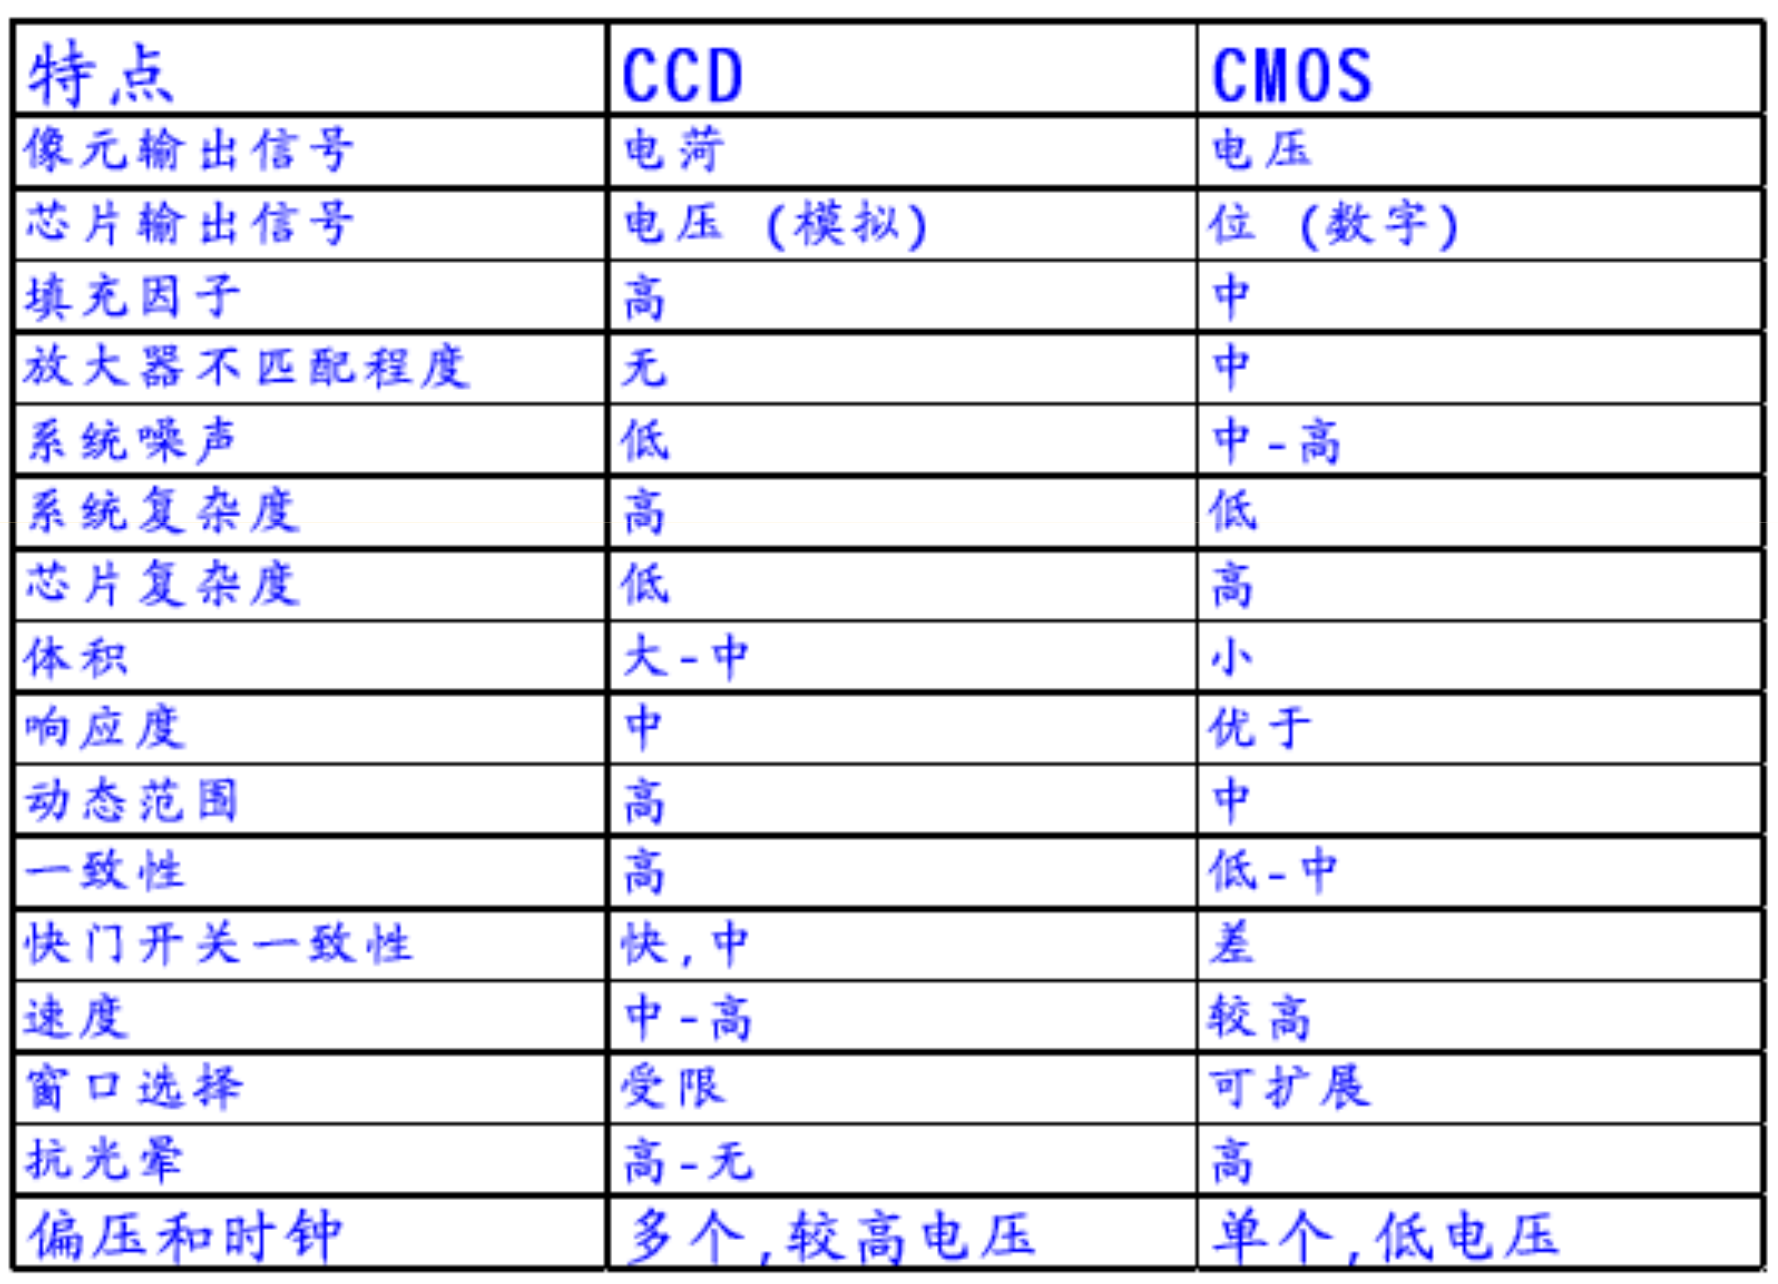
\includegraphics[scale=0.1]{imgs/CCD_CMOS.png}
\end{figure}

\subsection{快门}
Rolling Shutter 卷帘快门:逐行曝光,不适合拍摄运动物体,容易有拖影  \\
Global Shutter 全快门:一次曝光,适合拍摄运动物体

\subsection{光圈、焦距、景深}
光圈:$F=f/D$  \quad\quad $f:$ 焦距  \quad\quad  $D:$ 通光孔径  \\
$F$值越小,光圈越大  \\
光圈越小,景深越大;光圈越大,景深越小  \\
焦距越小,景深越大;焦距越大,景深越小  \\
被摄物越远,景深越大;被摄物越近,景深越小  \\
焦距越小,视场越大;焦距越大,视场越小


\section{光源}

\subsection{灰度照明技术}
\subsubsection{二值化处理}
\subsubsection{照明方式}
直射照明、漫射照明、透射照明、偏光照明  \\
偏光镜可以消除强反射光线和散射光,使光线变得柔和

\subsection{彩色照明技术}
光照颜色与物体颜色相同,则在二值图像中光将被明亮反射,显示为白色  \\
光照颜色与物体颜色互补,则在二值图像中光将被吸收,显示为黑色  \\
互补色:红+绿=黄,互补于蓝;红+蓝=紫,互补于绿;绿+蓝=青,互补于红

\subsection{照明方式}
直射方式、低角度方式、条形方式、聚光方式、平面环形方式、圆拱形方式、同轴方式、平行光、透射方式


\section{图像预处理}

\subsection{空域滤波}
均值滤波:会使图像模糊,尤其是边缘轮廓  \\
中值滤波:可有效抑制随机脉冲噪声(椒盐噪声)

\subsection{频域滤波}
图像中灰度变化缓慢的部分对应低频,图像的细节和边缘轮廓等灰度突变区域对应高频。  \\
通过低通滤波器可以滤除高频部分,实现降噪。常用的低通滤波器有高斯低通滤波器、巴特沃思低通滤波器、指数形低通滤波器等


\section{数学形态学}

\subsection{膨胀}
\ding{172} 将核的原点移至原图中的某一点  \\
\ding{173} 对原图和核求并集  \\
\ding{174} 对原图中的所有点重复上述操作  \\
\begin{figure}[htb]
    \centering
    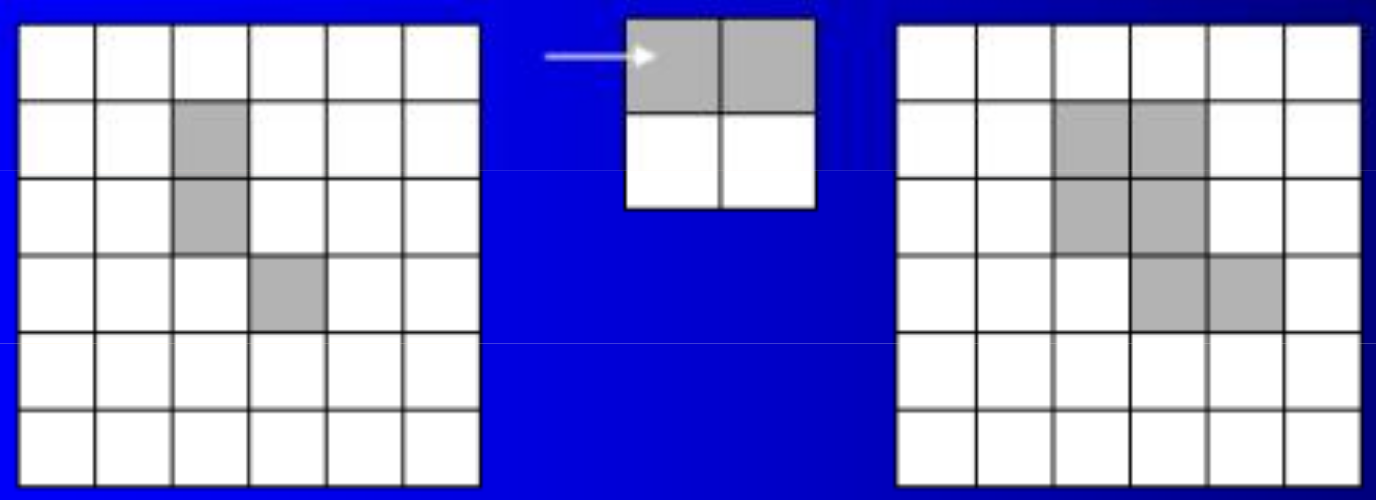
\includegraphics[scale=0.1]{imgs/dilate.png}
\end{figure}

\subsection{腐蚀}
用$B$腐蚀$A$得到的是$B$完全包括在$A$中时$B$的原点位置的集合。  \\
腐蚀可以把小于核的细节(如毛刺)去除,也可以将两个有细小连通的部分分开。
\begin{figure}[htb]
    \centering
    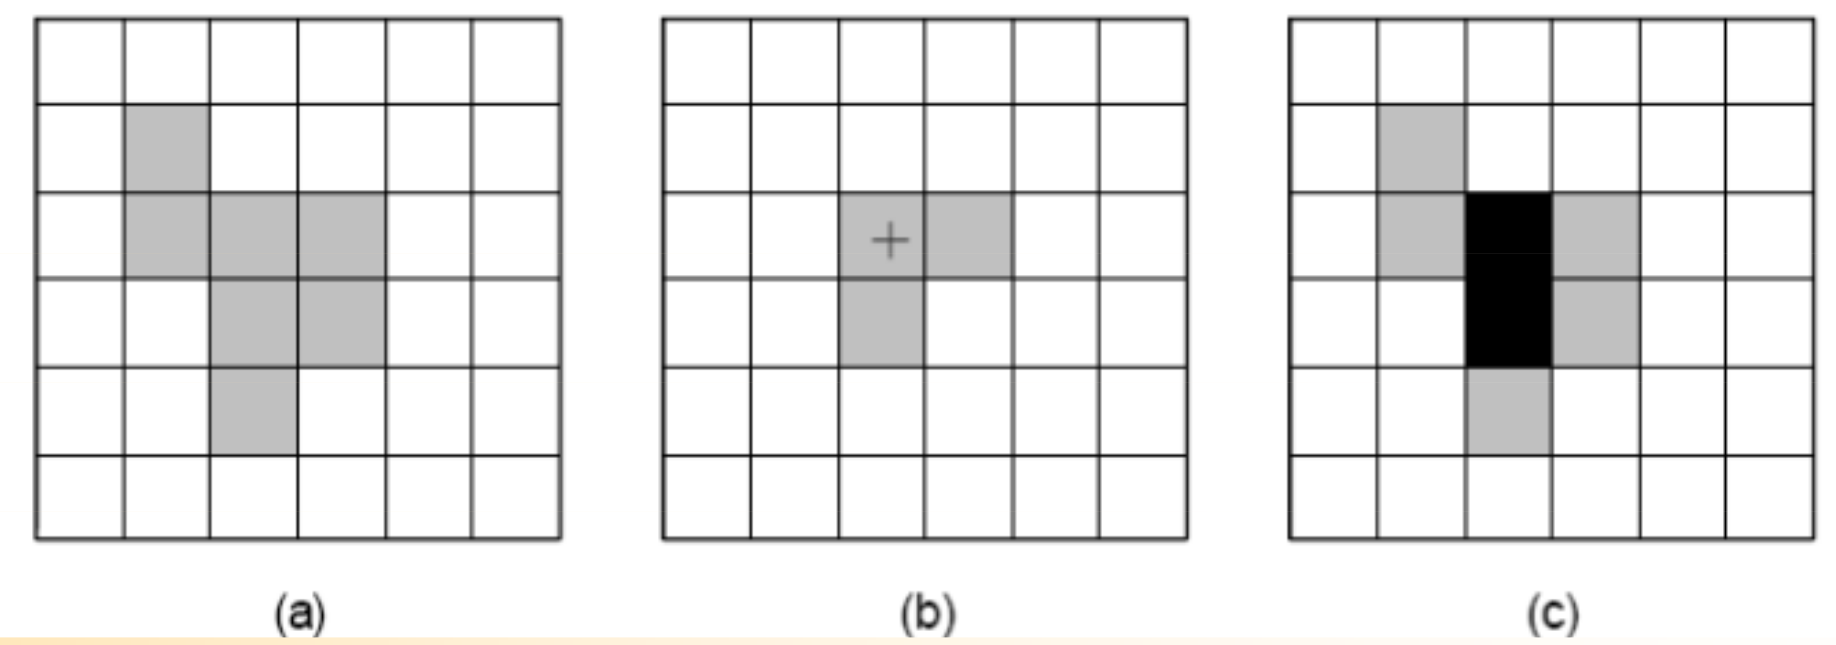
\includegraphics[scale=0.1]{imgs/erode.png}
\end{figure}

\subsection{开运算}
先腐蚀再膨胀。使图像的轮廓变得光滑,断开狭窄的间断,消除细的突出物。

\subsection{闭运算}
先膨胀再腐蚀。同样使轮廓变得光滑,但主要是消除长而细的鸿沟、小的孔洞,并填补轮廓线中的裂痕。

\subsection{形态学的应用}

\subsubsection{边界提取}
先腐蚀,然后用原图减去腐蚀后的图像

\subsubsection{骨架}
\begin{figure}[htb]
    \centering
    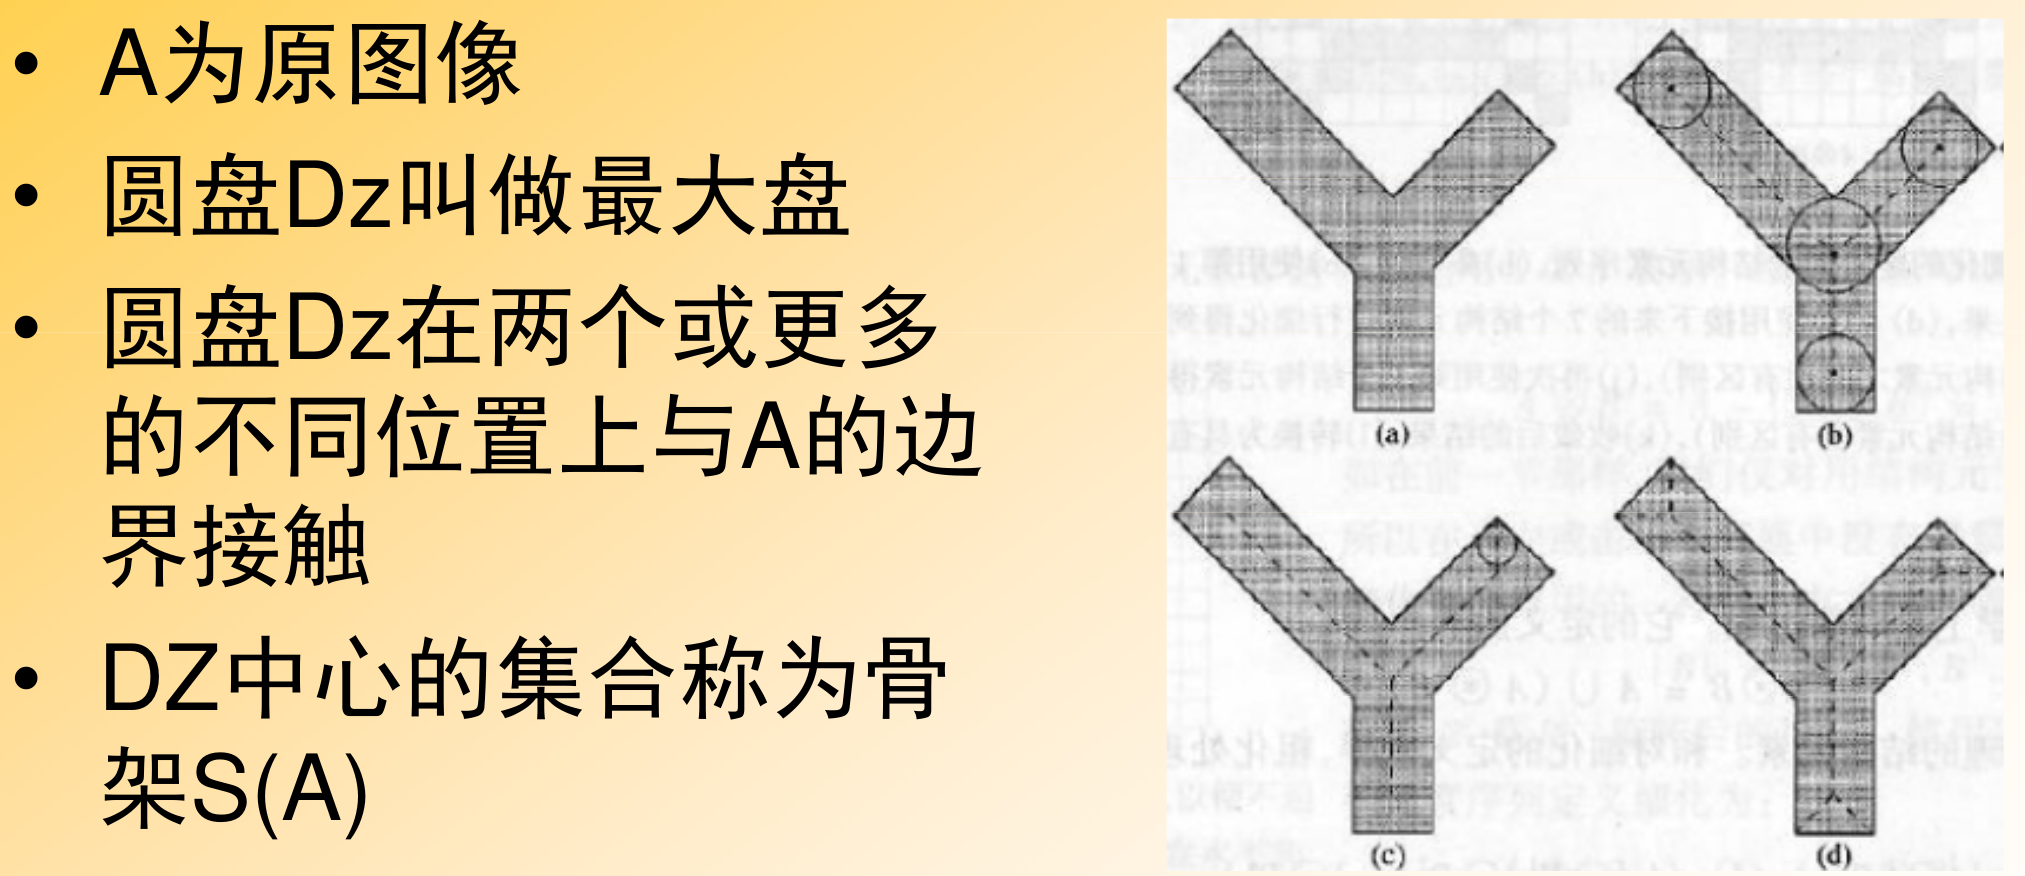
\includegraphics[scale=0.1]{imgs/bones.png}
\end{figure}

\subsection{灰度形态学}

\subsubsection{灰度膨胀}
将核的原点移至原图中某点$a$,在核的范围内将原图各点的灰度值与核各点的灰度值相加,取最大值作为$a$新的灰度值。
\begin{figure}[htb]
    \centering
    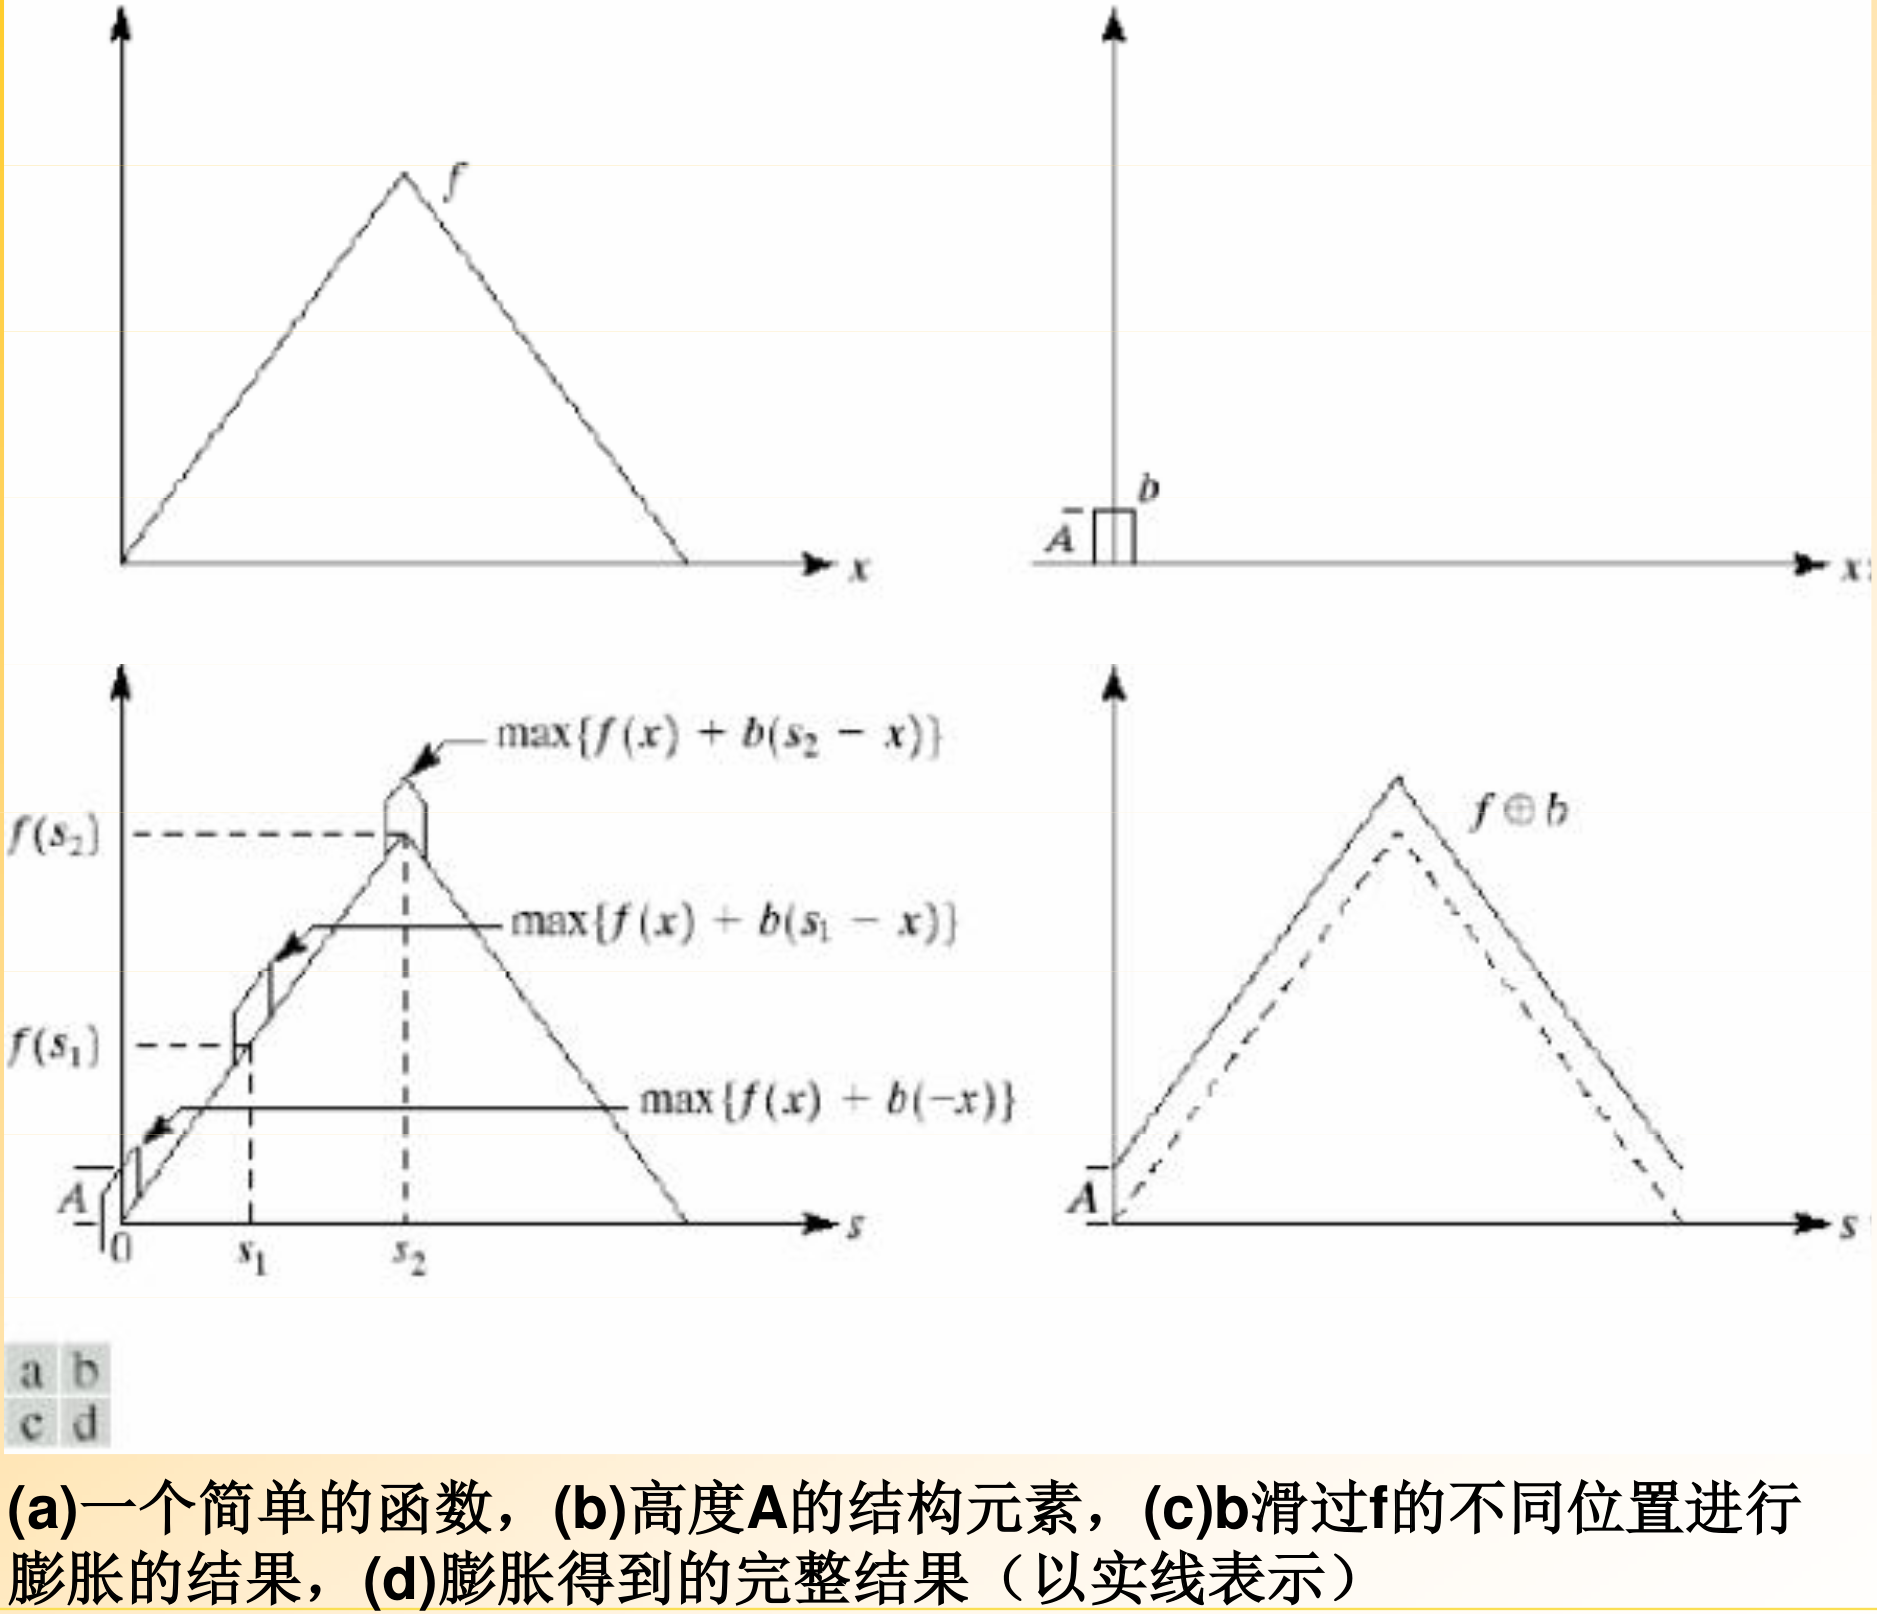
\includegraphics[scale=0.1]{imgs/gray_dilate.png}
\end{figure}

\subsubsection{灰度腐蚀}
类似于灰度膨胀,只不过是取原图灰度减核灰度的最小值。
\begin{figure}[htb]
    \centering
    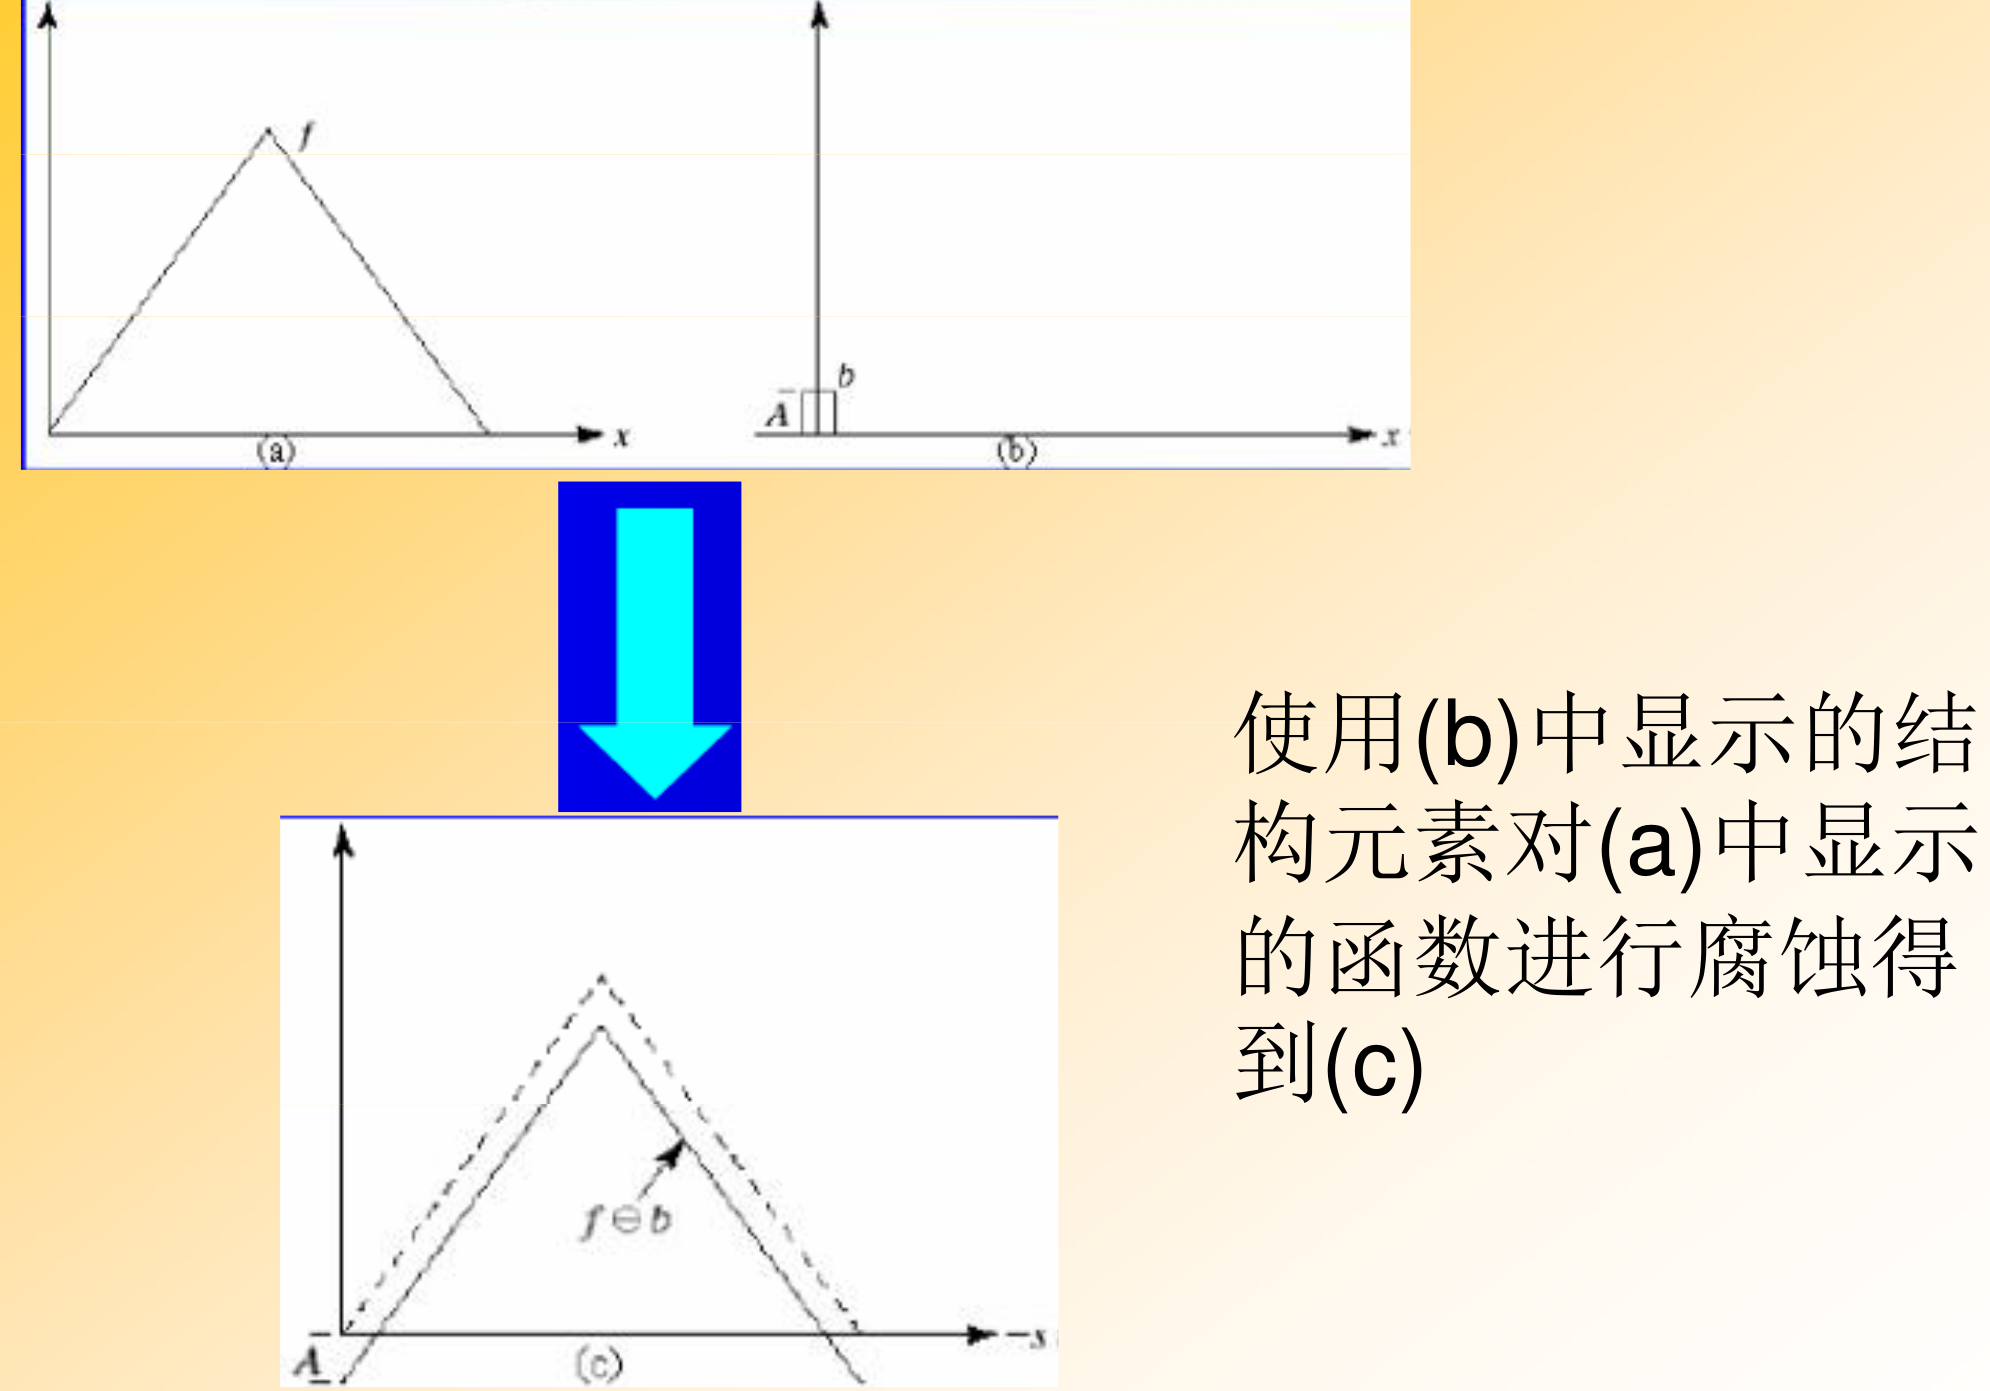
\includegraphics[scale=0.1]{imgs/gray_erode.png}
\end{figure}

\subsubsection{灰度开运算和灰度闭运算}
示例:电路板去除文字保留线路、机场跑道检测等


\section{边缘检测}

\subsection{边缘}
一阶导数可以用于检测图像中的一个点是否是边缘的点(灰度不变时一阶导数为零)
\begin{figure}[htb]
    \centering
    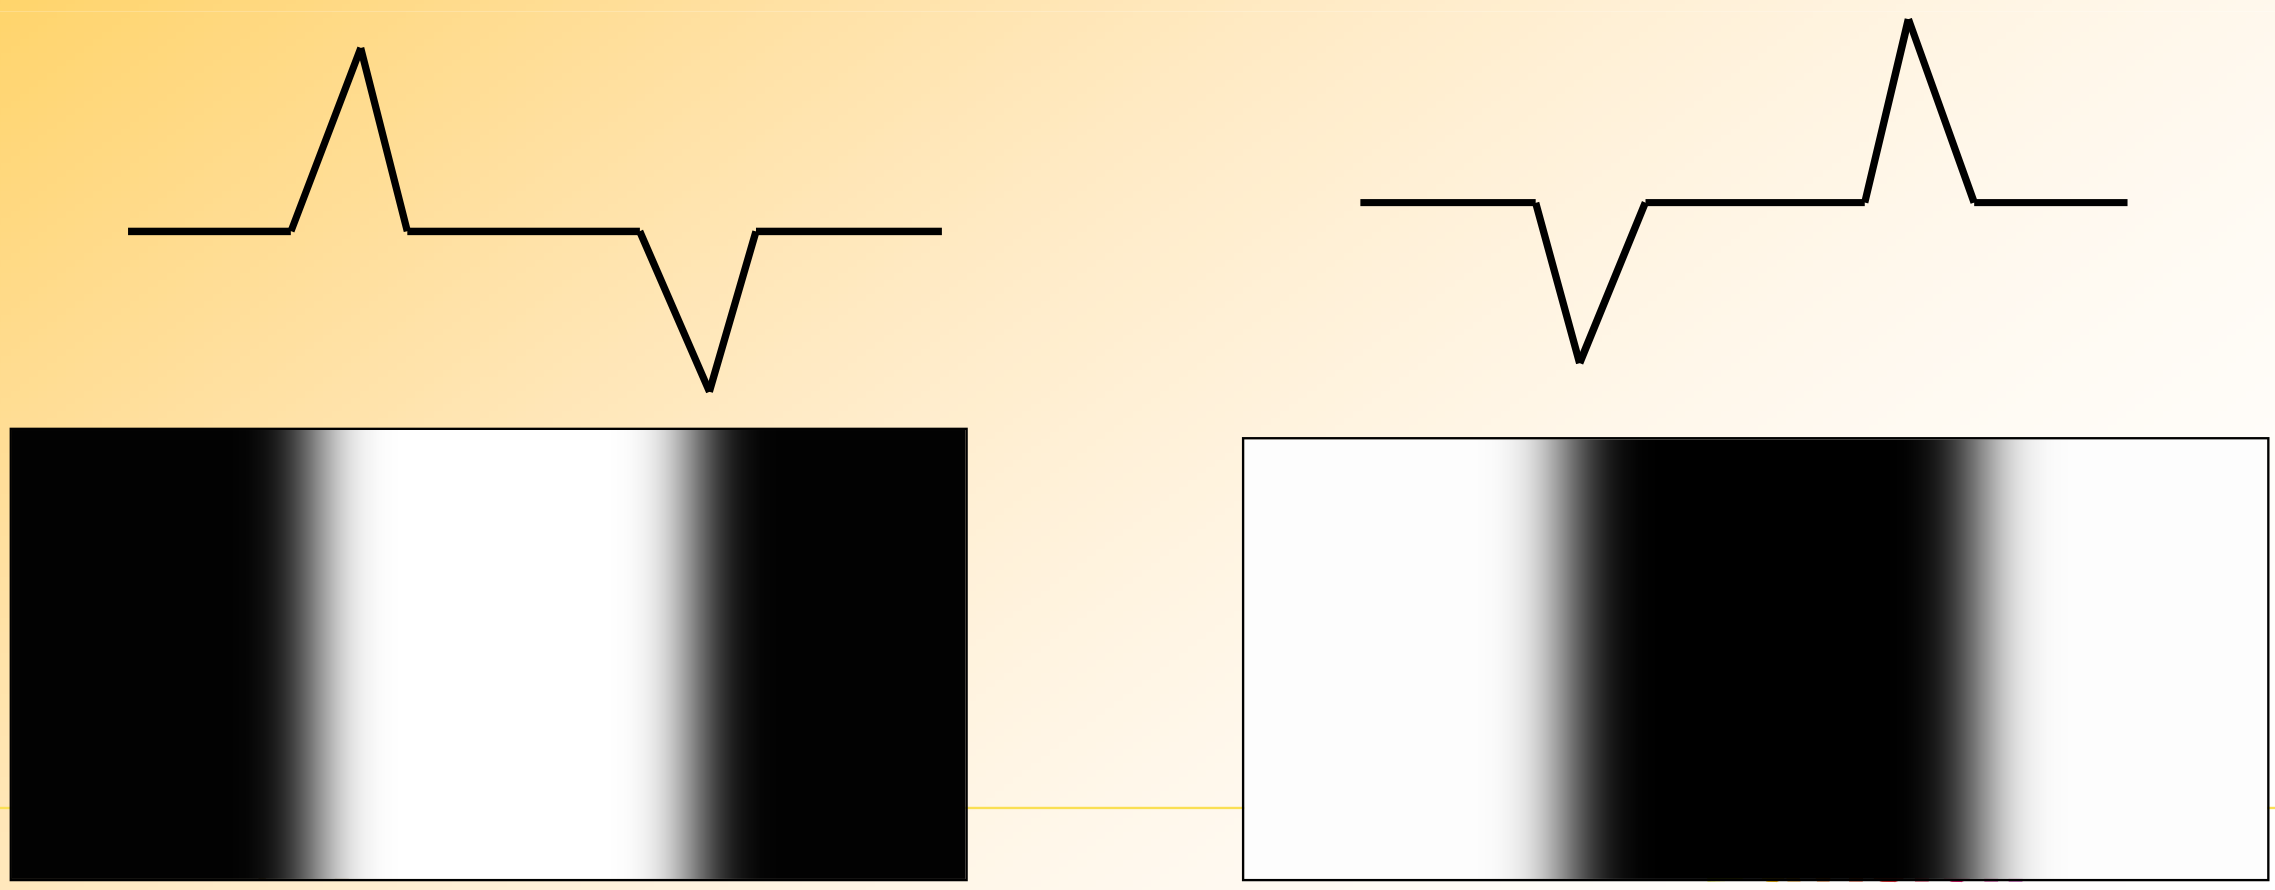
\includegraphics[scale=0.1]{imgs/edge_1.png}
\end{figure}
\\
二阶导数的符号可以用于判断一个边缘像素在边缘亮的一边还是暗的一边(正$\to$亮,负$\to$暗)
\begin{figure}[htb]
    \centering
    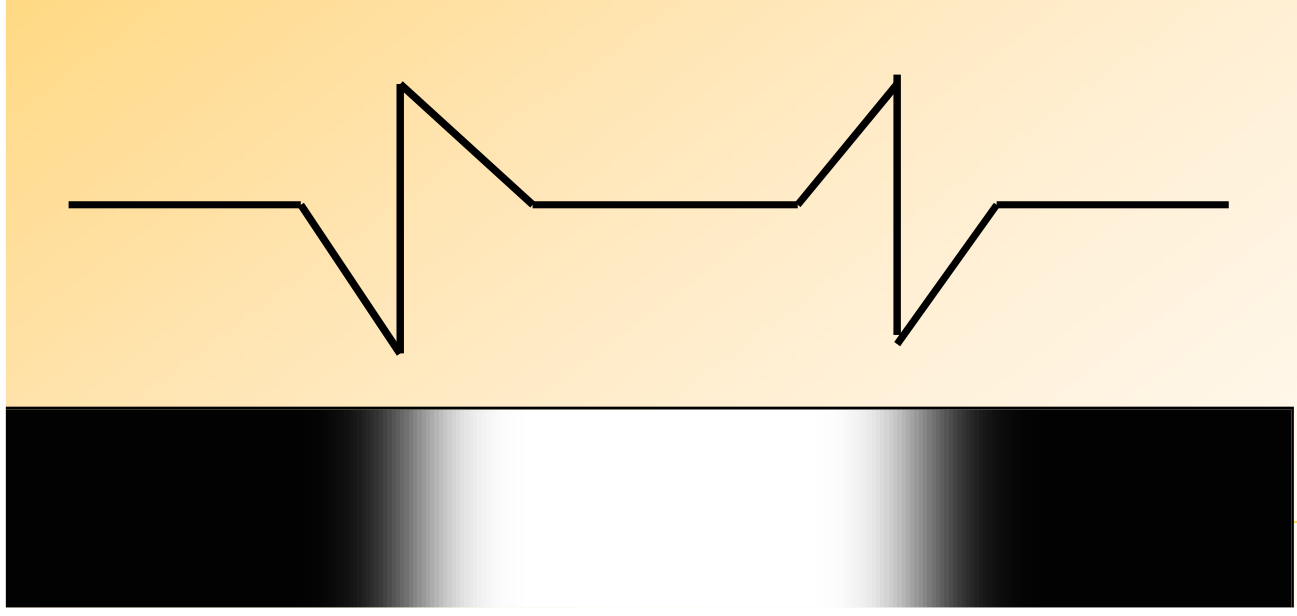
\includegraphics[scale=0.1]{imgs/edge_2.png}
\end{figure}

\subsection{边缘检测算子}

\subsubsection{梯度算子}
Roberts算子(2$\times$2模板)、Prewitt算子(3$\times$3模板)、Sobel算子(3$\times$3模板,增大中心点的权重)

\subsubsection{拉普拉斯算子}
对噪声敏感,容易产生双像素边缘

\subsubsection{Canny算子}
\begin{figure}[htb]
    \centering
    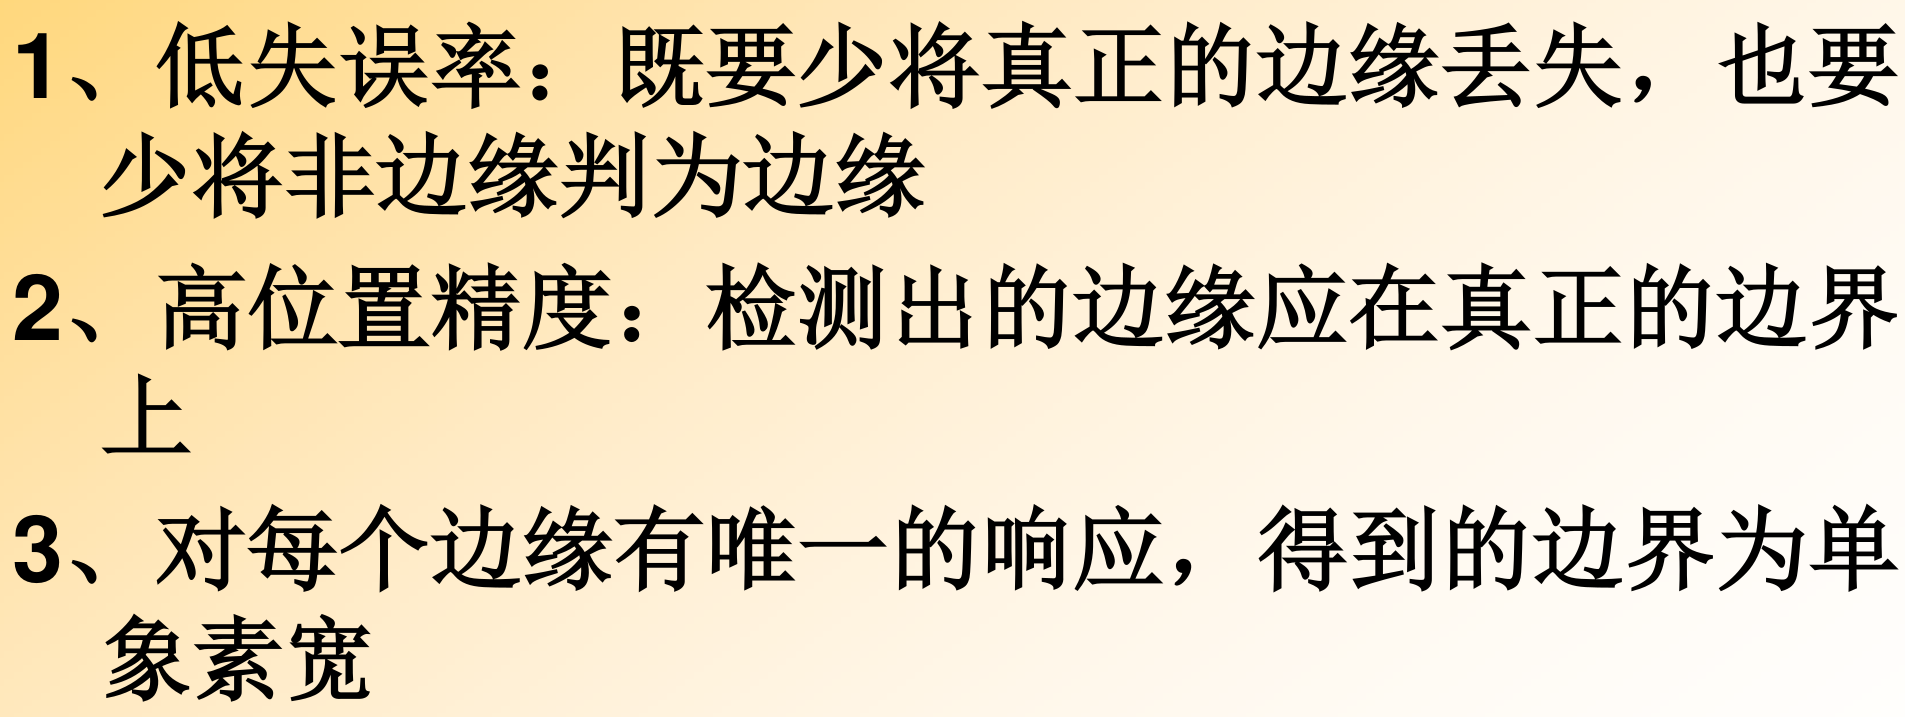
\includegraphics[scale=0.1]{imgs/canny.png}
\end{figure}


\section{图像分割}

\subsection{直方图}
图像中不同灰度值的像素所占的比例。  \\
若直方图呈现双峰分布,可取一个介于两峰之间的阈值分离前景和背景。
\begin{figure}[htb]
    \centering
    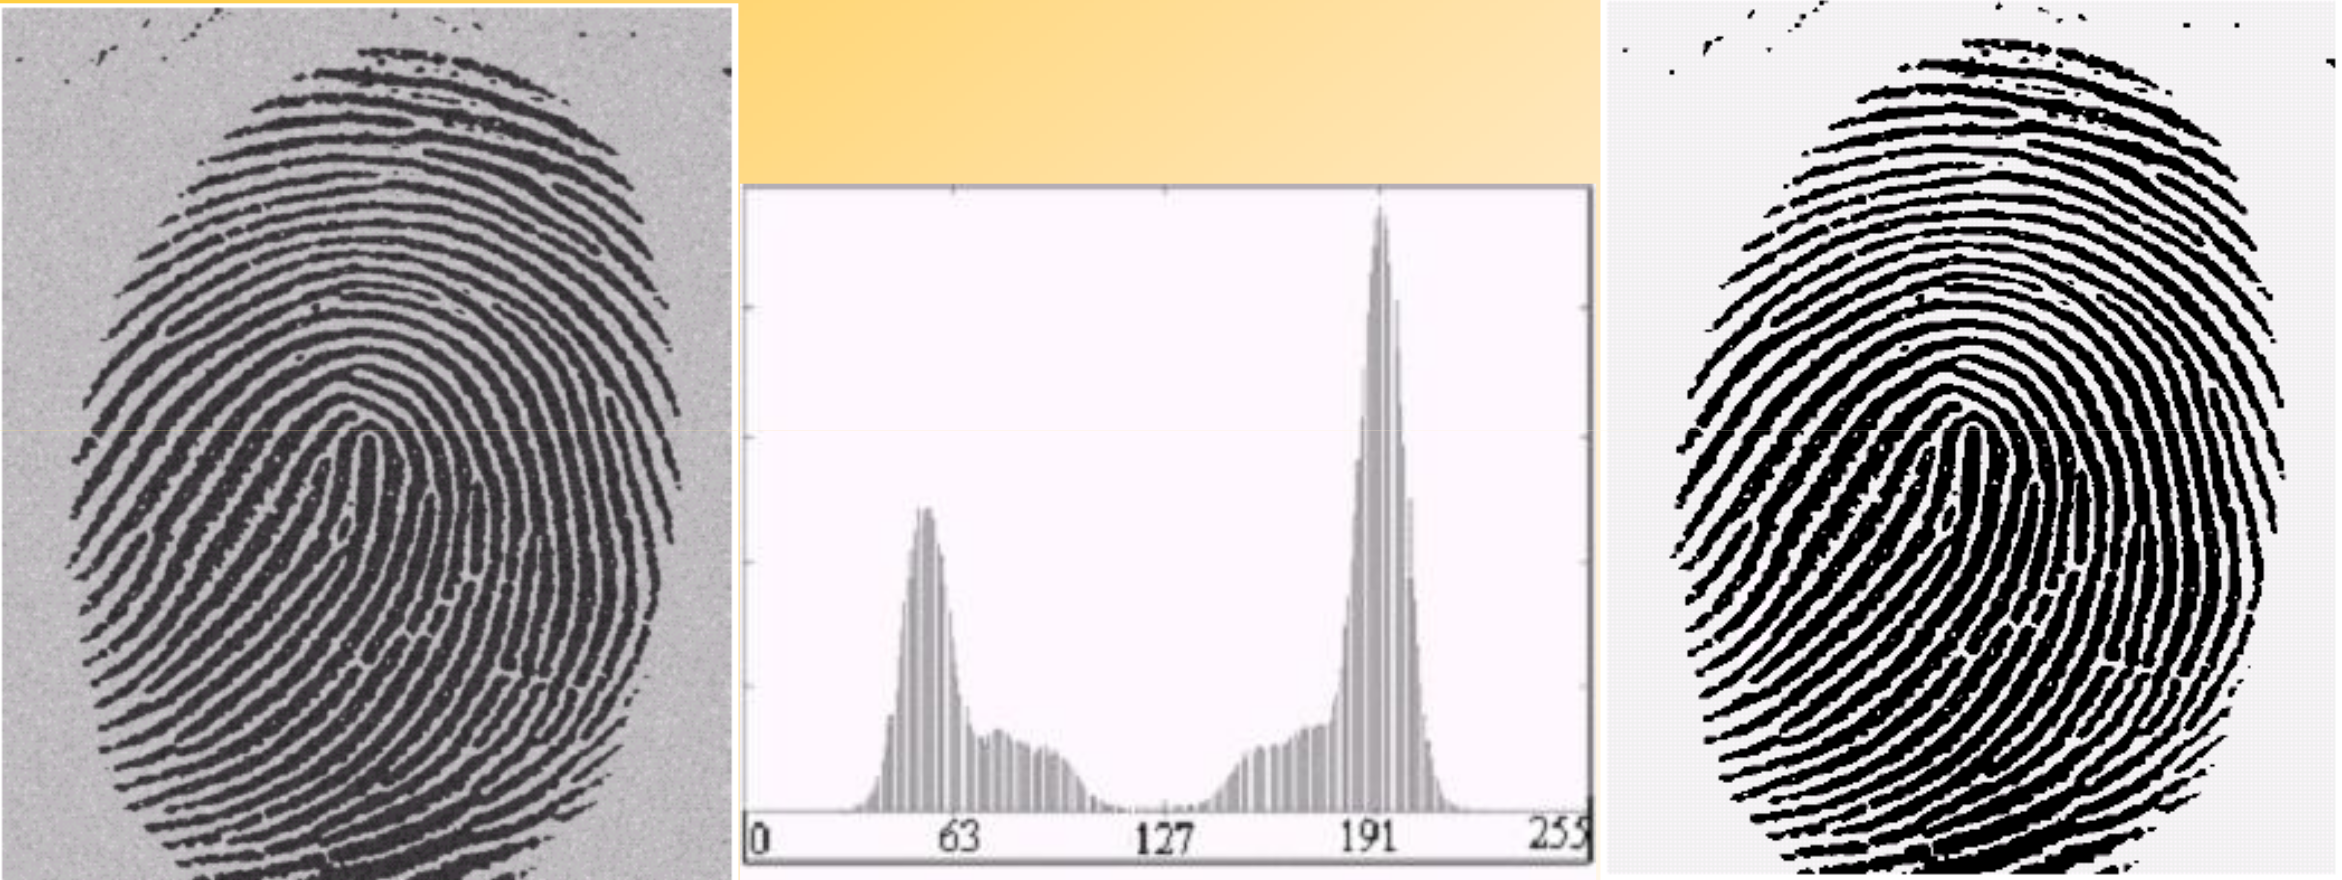
\includegraphics[scale=0.1]{imgs/bimodal.png}
\end{figure}

\subsection{多阈值分割}

\subsection{灰度均衡}
将原图的灰度范围映射到新的范围,增大对比度。具体方法包括线性均衡、对数均衡、指数均衡等

\subsection{局部阈值}
先进行单阈值分割,然后将分割后的结果作为种子,在原图中生长(灰度相近的视为同一物体)


\section{尺寸测量}

\subsection{点检测}
用空域的高通滤波来检测孤立点。
\begin{figure}[htb]
    \centering
    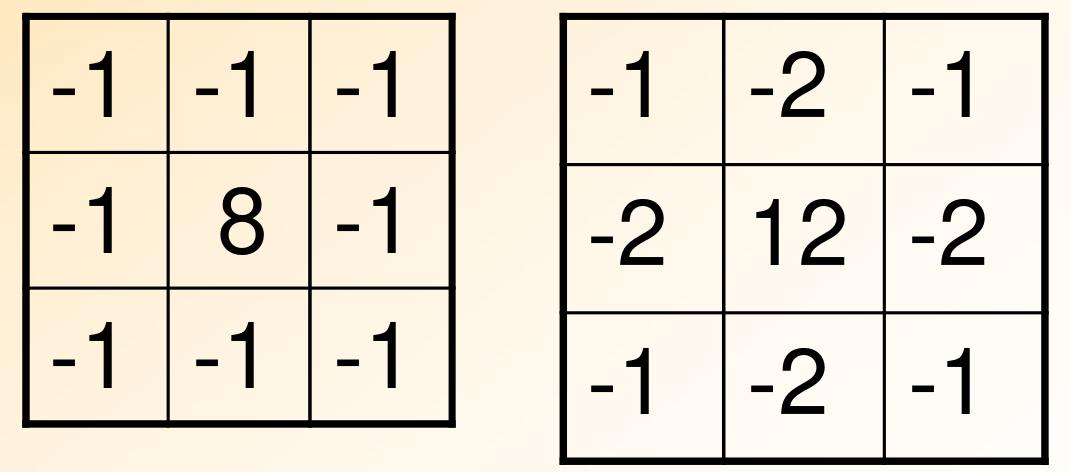
\includegraphics[scale=0.1]{imgs/dot_det.png}
\end{figure}

\subsection{线检测}
Hough变换
\begin{figure}[htb]
    \centering
    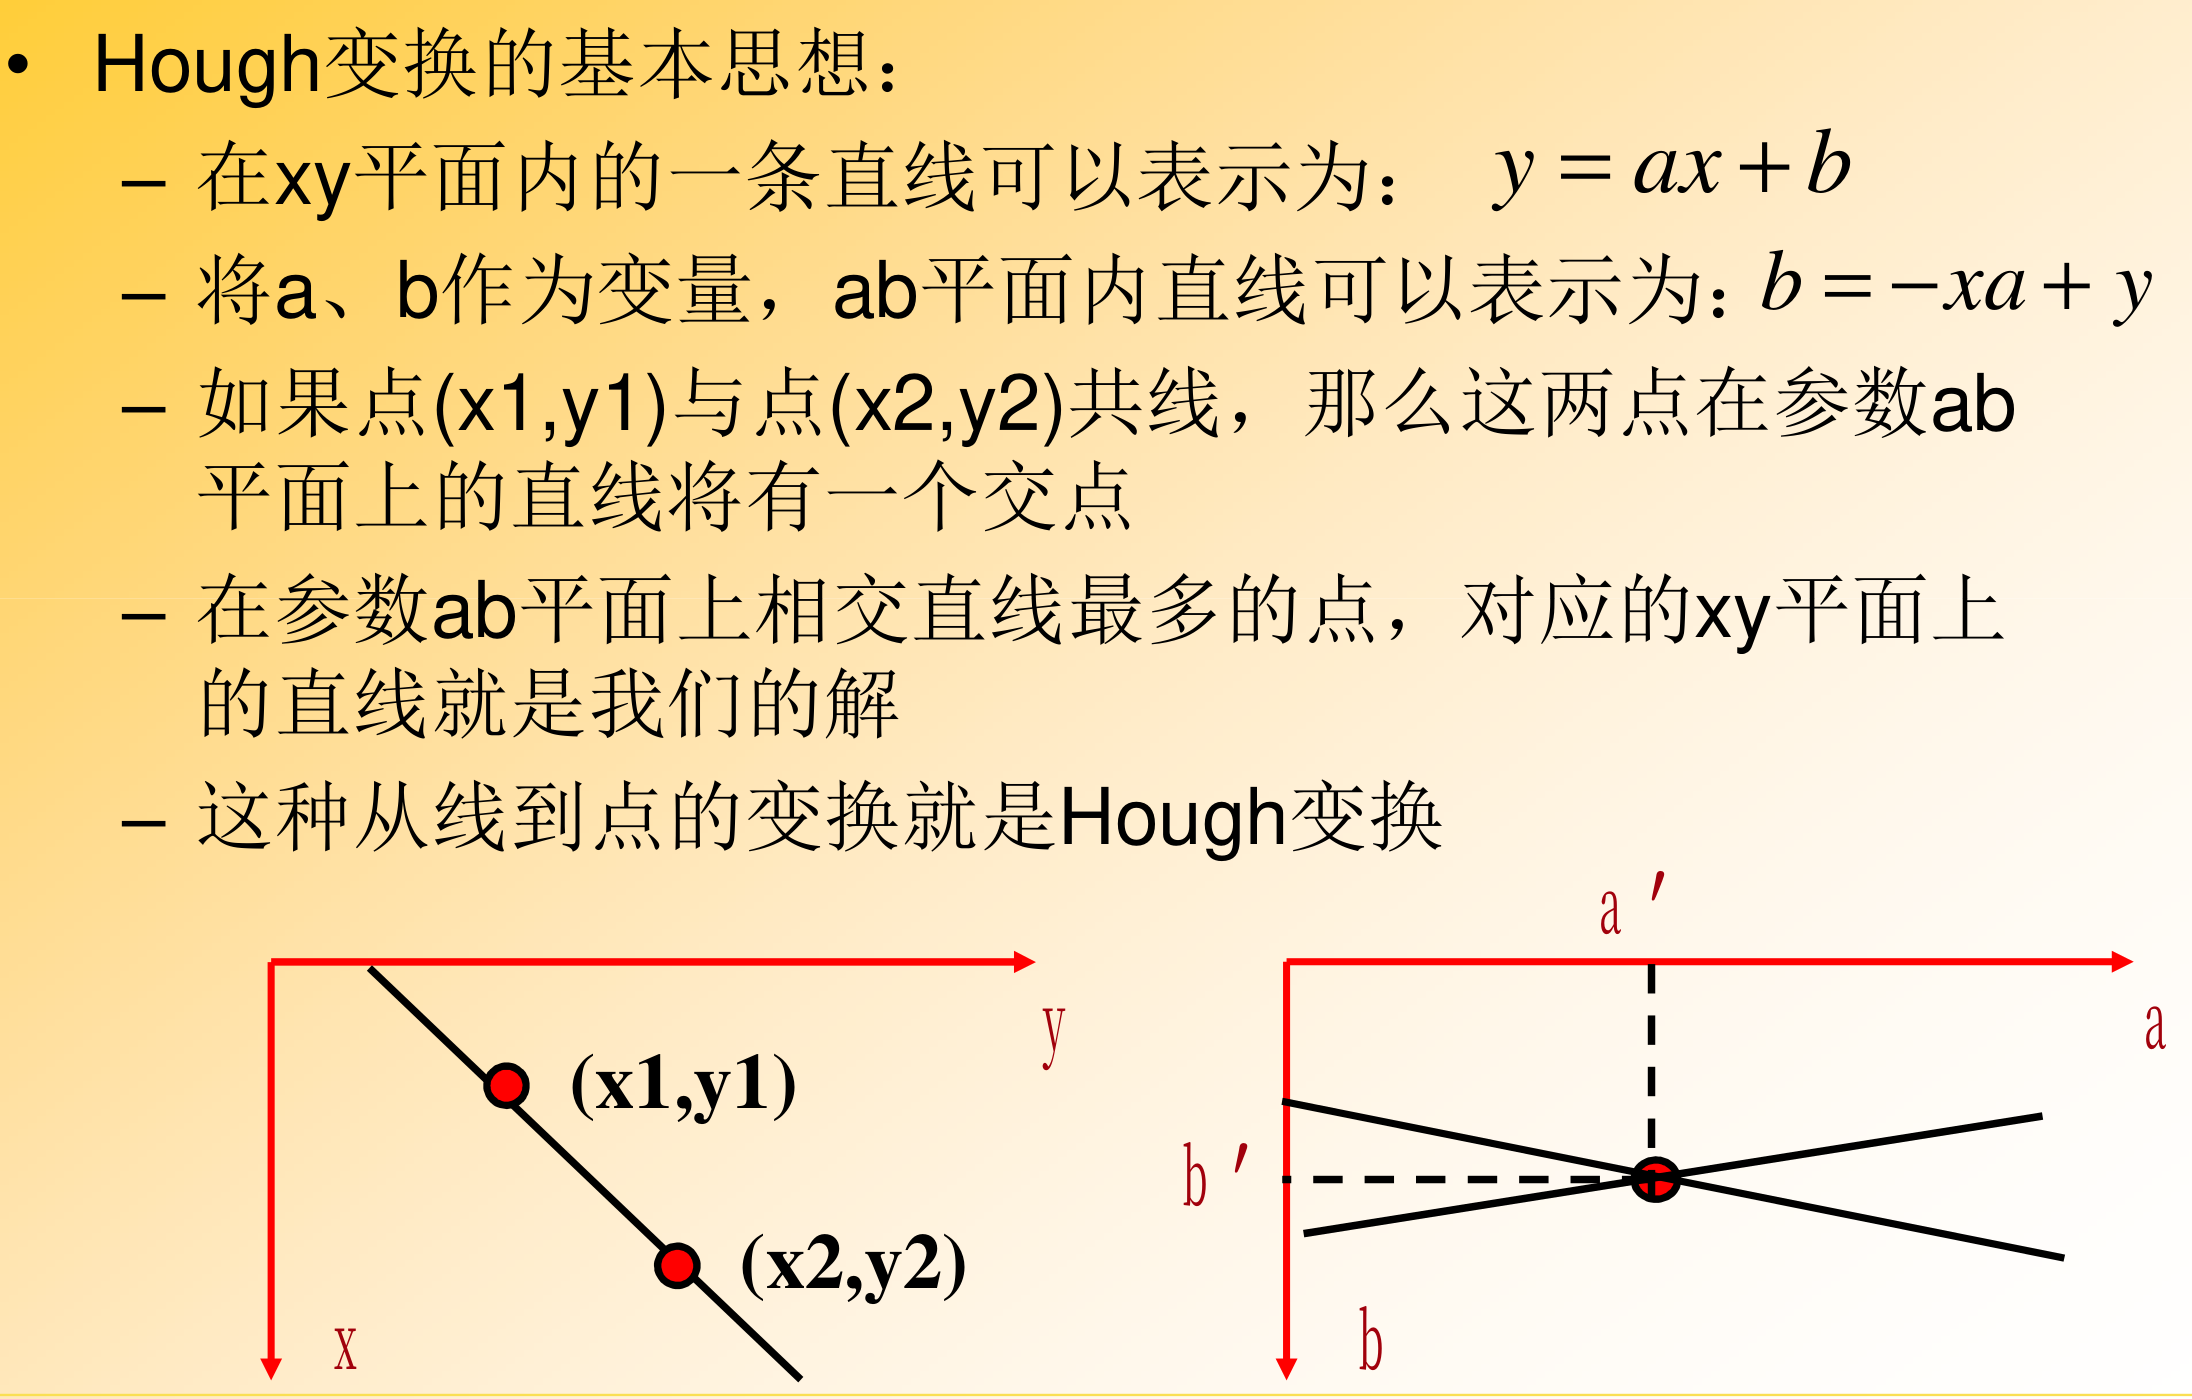
\includegraphics[scale=0.1]{imgs/hough.png}
\end{figure}
\\
由于垂直直线的斜率$a$无穷大,一般用极坐标形式 $\rho = xcos\theta + ysin\theta$  \\
除了检测直线外,Hough变换也可用于检测曲线,如圆、椭圆等。

\subsection{间距测量}
关键是检测到准确的边缘。

\subsection{角度检测}


\section{图像变换}

\subsection{反转变换}
$s=L-1-r$ \qquad 适用于增强嵌入于暗区域中的白色或灰色细节

\subsection{对数变换}
$s=clog(1+r)$  \qquad  适用于增强图像中低灰度的部分

\subsection{幂律(伽马)变换}
$s=cr^\gamma$  \qquad  当$\gamma < 1$时增强低灰度部分,当$\gamma > 1$时增强高灰度部分

\subsection{分段线性变换}
对于不同的灰度范围采用不同的线性变换,从而增强特定的灰度范围,增大对比度

\subsection{直方图均衡化}
增大对比度

\subsection{仿射变换}
用一个矩阵对原图像进行平移、旋转、放缩。
\begin{figure*}[htb]
    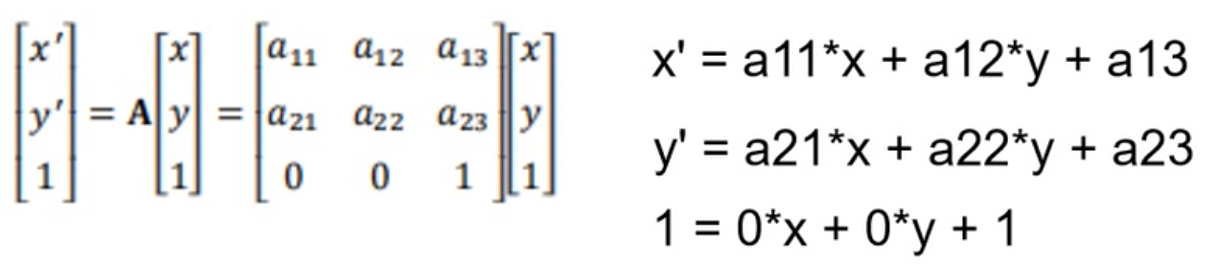
\includegraphics[scale=0.1]{imgs/affine.png}
    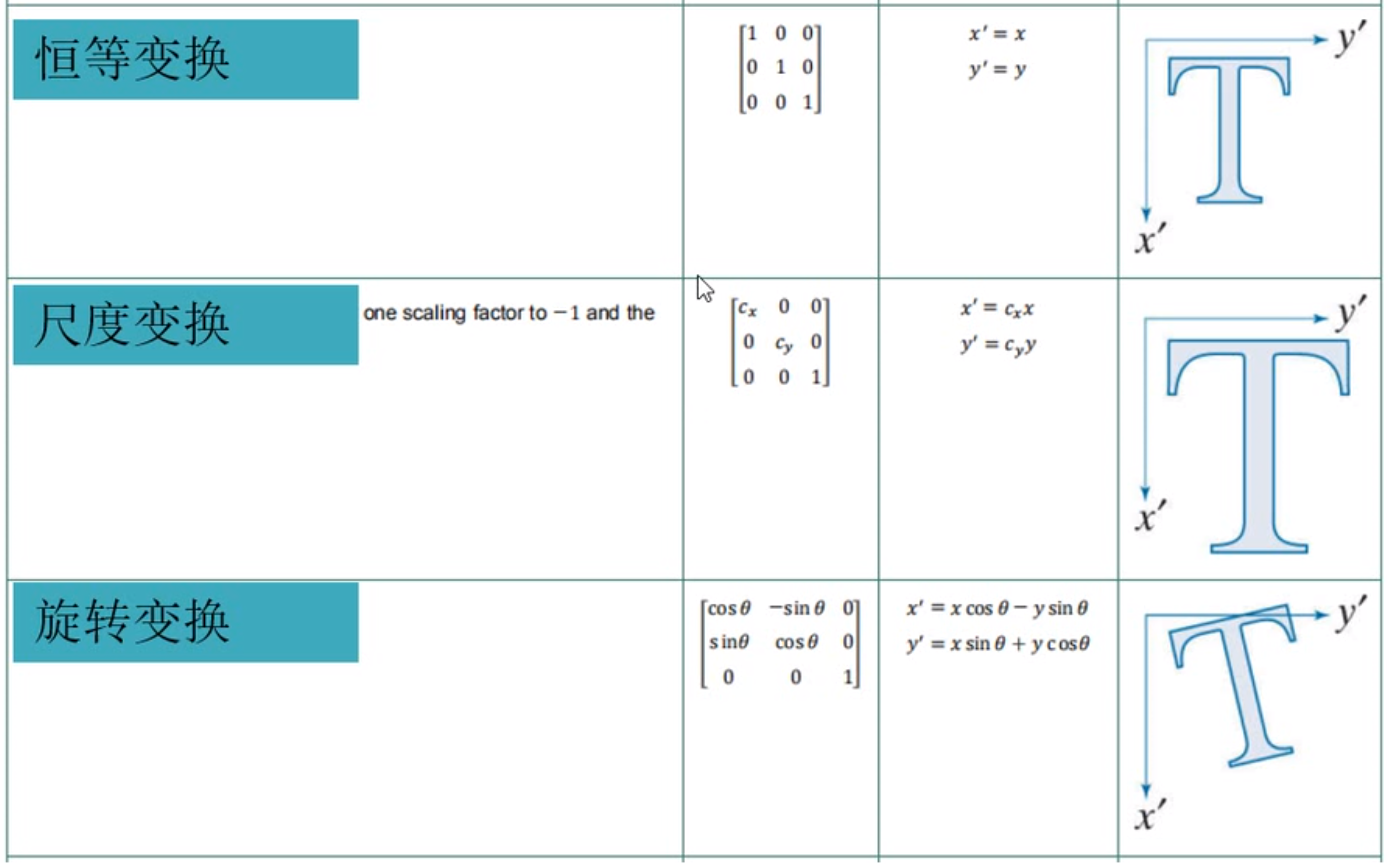
\includegraphics[scale=0.1]{imgs/affine_1.png}
    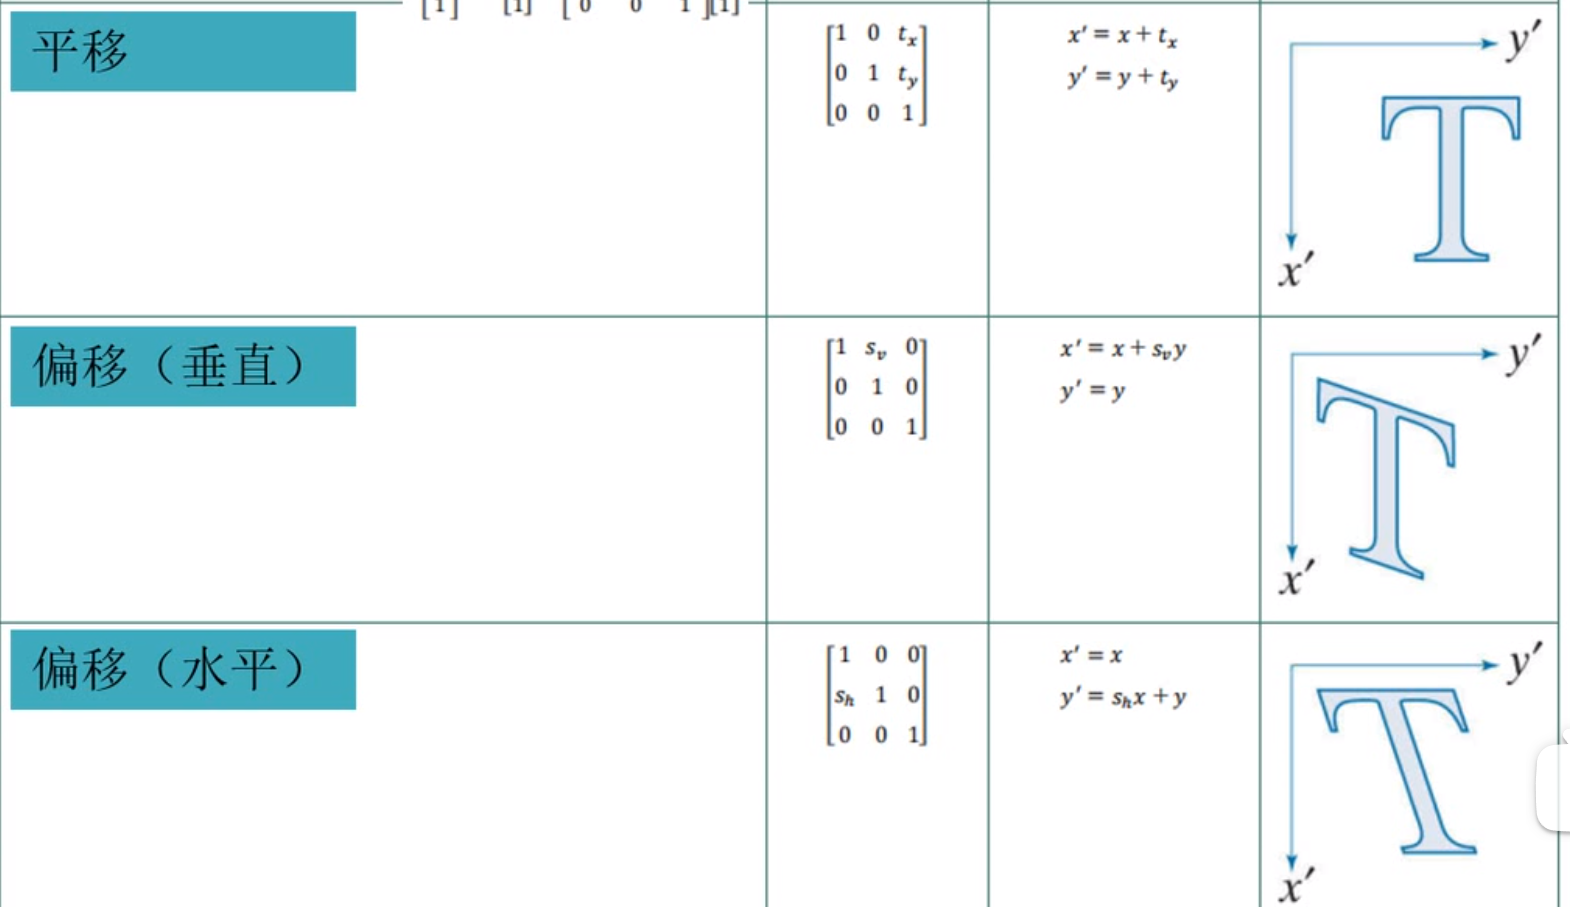
\includegraphics[scale=0.1]{imgs/affine_2.png}
\end{figure*}


\section{3D视觉}

\subsection{激光测距原理}
$z=\frac{b*f}{d}$  \qquad  $z$:待测距离 \quad $b$:基线 \quad $f$:焦距 \quad $d$:光斑与CMOS中心的距离
\begin{figure}[htb]
    \centering
    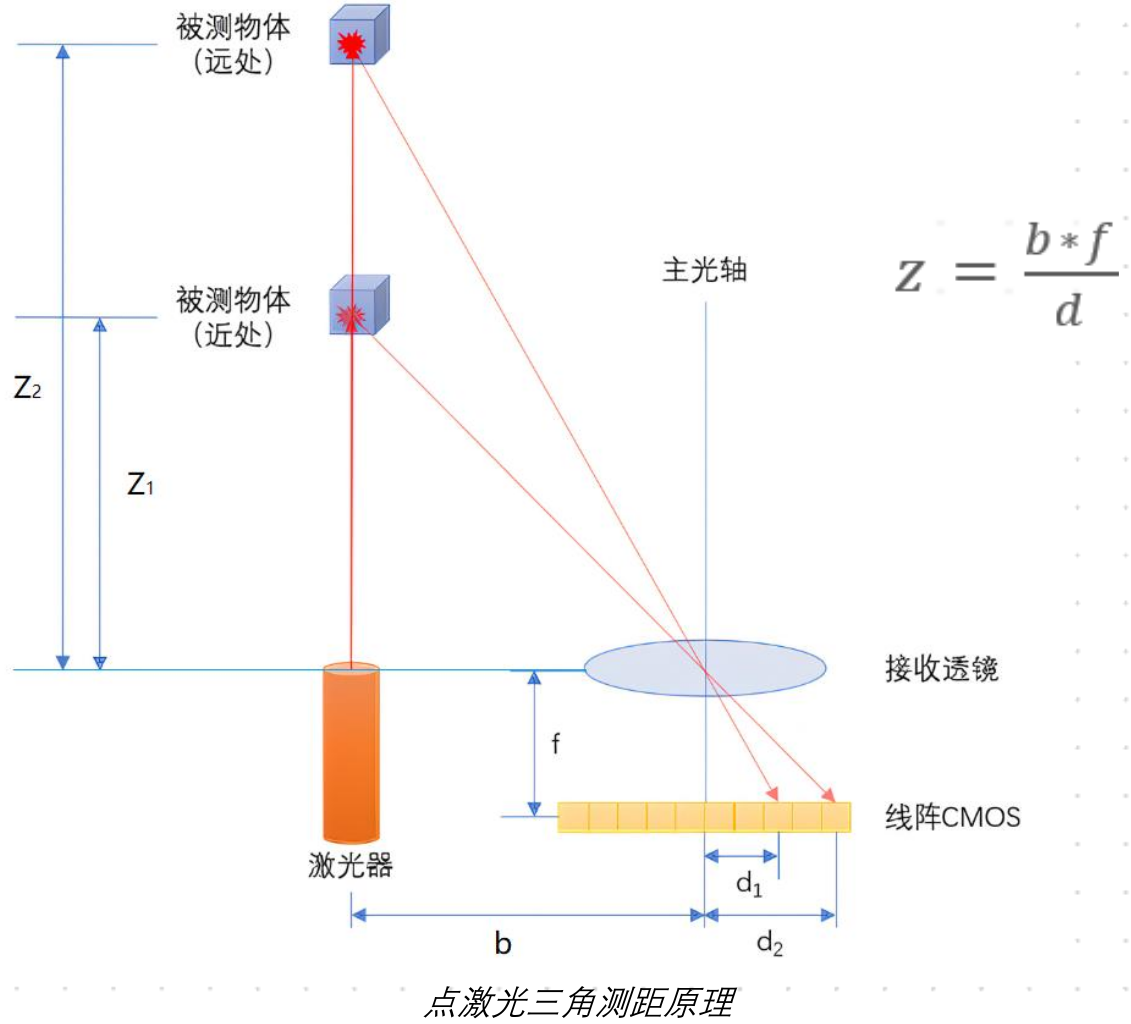
\includegraphics[scale=0.15]{imgs/zbfa.png}
\end{figure}

\subsection{结构光}

\subsubsection{散斑结构光}
投射编码散斑到物体上。

\subsubsection{条纹结构光}
投射多张编码条纹图,对每条竖线唯一编码,最后对每条竖线利用激光测距原理进行求解。由于需要多次投影和拍摄,速度较慢。
\begin{figure}[htb]
    \centering
    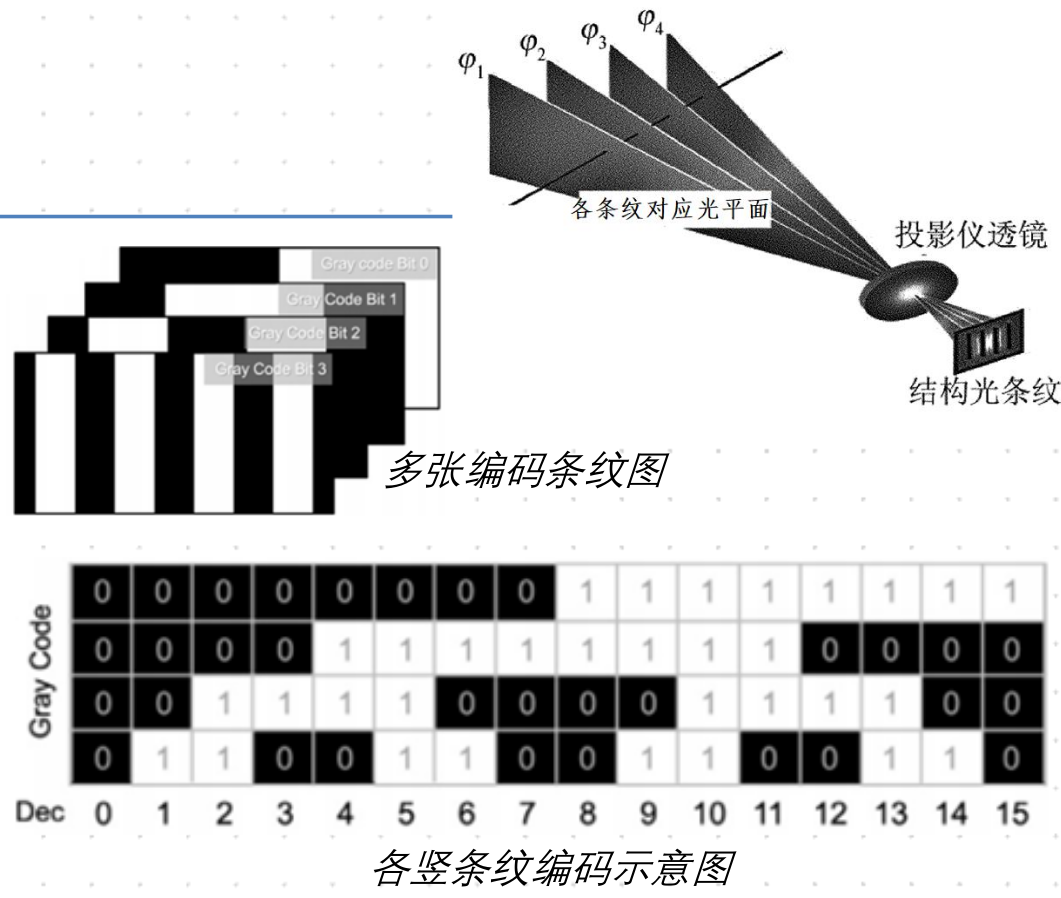
\includegraphics[scale=0.1]{imgs/tiaowen.png}
\end{figure}

\subsection{双目立体视觉}
提取左右两张图像中的特征点,建立一一匹配关系,通过视差求解距离,计算量巨大,速度慢。

\subsection{TOF}

\subsubsection{测量原理}
$d = \frac{\Delta t * c}{2}$  \\
计算量很小,速度快,但精度较低,一般在cm量级。

\subsubsection{两种方式}
dTOF:直接测量时间,测量精度主要受限于时钟的精度。  \\
iTOF:通过测量发射波和接受波之间的相位差间接测量时间。

\subsection{小结}
拍摄时间:条纹结构光(10+张)$>>$ 双目(2张)> 散斑(1张)> 线激光 > 点激光  \\
计算时间:双目 > 条纹结构光 > 散斑结构光 > 线激光 > 点激光  \\
温漂影响:双目好于TOF好于结构光(一般带投射器的方案受温漂影响较大)  \\
3D相机选型:相机视野、工作距离、成像时间、可靠性(防尘防水、振动防护等)、测量精度(绝对精度、
重复度)、分辨率、点云密度等


\section{相机标定}

\subsection{基本概念}
内参矩阵:从相机坐标系转换到图像坐标系,$3 \times 3$矩阵。  \\
外参矩阵:从世界坐标系转换到相机坐标系,$[R|T]$,$3 \times 4$矩阵。  \\
畸变参数:$(k_{1},k_{2},p_{1},p_{2}[,k_{3}[,k_{4},k_{5},k_{6}]])$,其中$k$为径向畸变
参数,$p$为切向畸变参数,一般取到$k_{3}$即可。

\subsection{手眼标定}
核心公式:$AX=XB$  \\
解释:对于ETH,可通过标定板$\to$机器人末端$\to$机器人底座和标定板$\to$相机$\to$机器人底座两条
路径列出标定板在机器人坐标系中的位置,其中相机坐标系和机器人底座的转换关系未知(待求),标定板和
机器人末端的坐标转换未知(可消去);对于EIH,可通过标定板$\to$机器人底座和标定板$\to$相机$\to$
机器人末端$\to$机器人底座两条路径列出标定板在机器人坐标系中的位置,其中相机坐标系和机器人末端的
转换关系未知(待求),标定板和机器人底座的坐标转换未知(可消去)。因此只要在两个不同位姿分别拍照,
消去标定板和机器人末端/底座的坐标转换,即可化为$AX=XB$形式,其中$X$为待求坐标转换。













\end{document}
